\documentclass[convert={
density=300,
outext=.png,
%preview=true,
%tikz=true
}]{standalone}
\usepackage{tikz}
\usetikzlibrary{chains,fit,shapes}
\usepackage{ulem}
\tikzstyle{tmtape}=[draw,minimum size=0.7cm]
\tikzstyle{large}=[minimum width=1.5cm]
\tikzstyle{current}=[draw=red!50]

\begin{document}
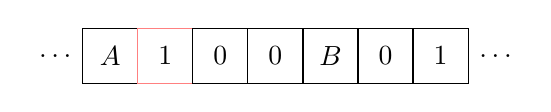
\begin{tikzpicture}
\begin{scope}[start chain=1 going right, node distance=-0.15mm]
    \node [on chain=1,tmtape,draw=none] {$\ldots$};
    \node [on chain=1,tmtape] {$A$};
    \node [on chain=1,tmtape,current] {1};
    \node [on chain=1,tmtape] {0};
    \node [on chain=1,tmtape] {0};
    \node [on chain=1,tmtape] {$B$};
    \node [on chain=1,tmtape] {0};
    \node [on chain=1,tmtape] {$1$};
    \node [on chain=1,tmtape,draw=none] {$\ldots$};
\end{scope}
\end{tikzpicture}
\end{document}

%%% Local Variables: 
%%% mode: latex 
%%% TeX-master: t
%%% End:
